% $Id: circuit.tex 9313 2021-08-07 16:45:06Z mskala $

%
% MSK 007 circuit explanation
% Copyright (C) 2017, 2021  Matthew Skala
%
% This program is free software: you can redistribute it and/or modify
% it under the terms of the GNU General Public License as published by
% the Free Software Foundation, version 3.
%
% This program is distributed in the hope that it will be useful,
% but WITHOUT ANY WARRANTY; without even the implied warranty of
% MERCHANTABILITY or FITNESS FOR A PARTICULAR PURPOSE.  See the
% GNU General Public License for more details.
%
% You should have received a copy of the GNU General Public License
% along with this program.  If not, see <http://www.gnu.org/licenses/>.
%
% Matthew Skala
% https://northcoastsynthesis.com/
% mskala@northcoastsynthesis.com
%

\chapter{Circuit explanation}

The MSK~007 Leapfrog Filter is a complicated circuit, and really
understanding how it works requires going quite deeply into the theory of
differential equations, complex variables, and so on.  I'm not going to go
that far.  This chapter presents \emph{three} intuitive descriptions (take
your pick!) of what goes on in a leapfrog filter in general, attempting to
use no more than basic calculus; as well as a practical summary of how the
MSK~007 in particular realizes the leapfrog design.  For more background,
read some standard textbooks on filter design, differential
equations, and complex variables; there are also some references footnoted
at appropriate points in this explanation.

%%%%%%%%%%%%%%%%%%%%%%%%%%%%%%%%%%%%%%%%%%%%%%%%%%%%%%%%%%%%%%%%%%%%%%%%

\section{Core topology}

The MSK~007's fifth-order leapfrog filter core consists of five active
integrators, each of which integrates the difference between the outputs of
the next and previous integrator in the sequence.  There is special handling
at the ends: the first one uses the filter input as its
otherwise-nonexistent ``previous'' neighbour, and the last one uses its own
output as its otherwise-nonexistent ``next'' neighbour.  Then there is also
an output mixer that combines the outputs of all five integrators in a fixed
proportion.  In principle, the circuit input could also be included as an
input to the output mixer, but in fact that is not done in the specific case
of the MSK~007.

{\centering\input{coretopo.tex}\par}

Keep this topology of the core in mind while reading the next sections, which
attempt to justify \emph{why} it is a useful way to build a filter core.

%%%%%%%%%%%%%%%%%%%%%%%%%%%%%%%%%%%%%%%%%%%%%%%%%%%%%%%%%%%%%%%%%%%%%%%%

\section{Calculus intuition}

This intuitive explanation is for readers with a more mathematical
inclination; read the ``analog electronics'' section below if you find
that approach easier to understand.  Note that here I'm going for easy
understandability, not rigour.

Suppose we want to build a filter that has a specific response to input
described by a differential equation, like this:
\begin{equation}
  Ax^{\mathrm{(v)}}+By^{\mathrm{(v)}}+Cy^{\mathrm{(iv)}}+Dy'''+Ey''+Fy'+Gy = 0 \, .
  \label{eqn:differential}
\end{equation}

The variables $x$ and $y$ represent the input and output, respectively. 
Both of those are functions of time ($x(t)$ and $y(t)$), and the primes and
Roman numerals represent taking multiple derivatives of them with respect to
time.  In words, \eqref{eqn:differential} says that some linear combination
of the fifth derivative of the input $x^{\mathrm{(v)}}$, and of all
derivatives of the output from $y$ up to $y^{\mathrm{(v)}}$, adds up to zero.

Exactly \emph{why} it makes sense to describe a filter's response that way,
and how we choose the coefficients $A$ through $G$ (all of which are
constant real numbers) to make the filter sound the way we want it to, are
beyond the scope of this explanation.  In very rough terms, we'll just say
that filters do tend to be well-described by this kind of equation---it's a
natural way to describe what a filter does---and having seven different
coefficients to choose means we have a lot of opportunities to tailor the
filter to respond in a way we want.  So with that in mind, just assume we
have somehow chosen coefficients for the differential equation such that a
filter behaving according to that equation would be a filter we would like
to build.  Now how can we build one?

First, it's more convenient to build electronic integrators than
differentiators, so let's take the integral of the differential equation,
five times, so there are no primes left.  I'll just write integral signs
instead of spelling out limits, constants, and the fact that all of these
are integrals over time:
\begin{multline}
  Ax+By+C\int y+D\iint y+E\iiint y \\ +F\iiiint y+G\iiiiint{} y = 0 \, .
  \label{eqn:integral}
\end{multline}

At this point we could actually turn it into a circuit.  Starting with the
signal $y$ coming from somewhere, we'd chain together five integrators
to compute each multiple integral up to $\iiiiint y$.  Given $x$
and all the integrals, what is left is just a single linear equation with
only one unknown, $y$; so we can build a constant-ratio linear mixer that
actually computes the value of $y$ to satisfy~\eqref{eqn:integral}.  That
value of $y$ is the circuit output, and it also loops back to supply the
value of $y$ to the input of the integrator chain.  The feedback allows the
circuit to solve the equation.

What I've just described is (one form of) a classical state-variable filter
with five state variables.  Note that what people usually call a
``state-variable filter'' in synthesizers is specifically a two-pole version
with some tricks to allow it to have multiple useful outputs.  This
five-pole state-variable filter is a little different, but both are examples
of the general state-variable technique.

There are some problems with actually building a multi-pole state variable
filter that way, however, notably that it's necessary to get the
coefficients exactly right or else the final output will be far from its
correct value.  By means of Laplace transforms and algebra, it is
possible to rearrange our equation into a system of equations in new
variables $v_1$, $v_2$, $v_3$, $v_4$, $v_5$ such that it has the same
solution as~\eqref{eqn:differential} but a different form:
\begin{equation}
  \begin{gathered}
  v_1 = H\int(x-v_2) \\
  v_2 = I\int(v_1-v_3) \\
  v_3 = J\int(v_2-v_4) \\
  v_4 = K\int(v_3-v_5) \\
  v_5 = L\int(v_4-v_5) \\
  y = Mx+Nv_1+Pv_2+Qv_3+Rv_4+Sv_5 \, .
  \end{gathered}\label{eqn:tridiagonal}
\end{equation}

One way of thinking of this is that it comes down to putting a matrix into
tridiagonal form.  Choosing values for the coefficients $H$ through $S$ is
complicated, but only a matter of arithmetic using formulas that have been
published in the academic literature.\footnote{Yichuang Sun, 2006, Synthesis
of Leap-Frog Multiple Loop Feedback OTA-C Filters, IEEE Transactions on
Circuits and Systems, Part 2: Express Briefs, 53, 9.} Every one of those
equations is something we can easily calculate with an analog computer: just
a scaled integral of the difference between two other signals for $v_1$
through $v_5$, or a linear mixture of signals for $y$ at the end.  There are
still five integrations being performed, but with multiple feedback
conenctions among them instead of just one master feedback connection from
the end back to the start.  The circuit solves the system of
equations~\eqref{eqn:tridiagonal}, which has the same solution
as~\eqref{eqn:differential} and~\eqref{eqn:integral}, so it also functions
as a filter with the desired response.

The important difference is that expressing the filter response in the
form~\eqref{eqn:tridiagonal} is more \emph{numerically stable}.  Small
errors in the coefficients don't have as much effect on the final output as
would be the case with the classical state-variable form.  As a rough
intuition, that is because any feedback tends to cancel out errors, but here
an error in one integrator's output loops back to its input after passing
through at most one other integrator, whereas in the classical design it
would go around the entire cycle through all the other integrators, causing
more damage.  So it is more likely that if we build a machine according
to~\eqref{eqn:tridiagonal}, it will actually work to compute the response we
want.

%%%%%%%%%%%%%%%%%%%%%%%%%%%%%%%%%%%%%%%%%%%%%%%%%%%%%%%%%%%%%%%%%%%%%%%%

\section{Analog electronics intuition}

If you're more comfortable thinking about components than differential
equations, this section may interest you.  Suppose we want to build
a traditional five-pole passive LC filter that looks like this:

{\centering\input{passivelc.tex}\par}

The component values would probably come from using a table of prototype
filters; that method and the math that goes into making the lookup
tables are beyond the scope of the current discussion.

We probably wouldn't actually build a filter using real capacitors and
inductors like that, especially not at audio frequencies, because inductors
suck.  They do not behave much like the mathematical model of what an
inductor is supposed to do, and so the filter will not really work well. 
Even if we tried, the necessary component values for audio frequencies would
probably lead to our needing inductors that are too physically large to be
practical.  Passive LC filters like the above are sometimes used in radio
applications, where the component values are more reasonable and it's
possible to make inductors that work acceptably, but for audio it's much
more common to do what we're about to: build an analog computer that
\emph{simulates} the passive LC circuit as if it were built with ideal
instead of real-life components.

Now, looking at the circuit diagram, let's assume all the impedance matching
has been magically done for us, so that the input looks to the source as if
it were a pure resistance.  The resistors shown on the diagram just
represent perfectly matched impedances; let's pretend they are each
1$\Omega$, which conveniently makes voltage and current through each one
equal.  We can describe the input signal then
equivalently as a voltage or a current; for convenience, use the current
$I_{\textrm{in}}$.  To understand the operation of this circuit we need to
be able to calculate the final output voltage $V_3$, and it'll help to
compute all the other voltages and currents in between the input and output.

Current feeding through the input resistor splits into current through
$L_1$, named $I_1$, and current through $C_1$, which doesn't have a name but
by Kirchoff's Current Law must be equal to $I_{\textrm{in}}-I_1$.  A
capacitor's voltage is just the integral of the current through it, scaled
to the inverse of the capacitance, so we have:
\begin{equation*}
  V_1 = \frac{1}{C_1} \int (I_{\textrm{in}}-I_1) \, .
\end{equation*}

Note that we can decide that equation is true, even though we haven't
actually calculated the value of $I_1$ yet.

Computing the current $I_1$ through $L_1$ is next.  The current through an
inductor is just the integral of the voltage applied to it---apply a fixed
voltage for a period of time and the current increases linearly.  So we can
write:
\begin{equation*}
  I_1 = \frac{1}{L_1} \int (V_1-V_2) \, .
\end{equation*}

The same considerations give expressions for $V_2$ and $I_2$:
\begin{gather*}
  V_2 = \frac{1}{C_2} \int (I_1-I_2) \\
  I_2 = \frac{1}{L_2} \int (V_2-V_3) \, .
\end{gather*}

The expression for the final voltage $V_3$ is a little special because we
need to use the current exiting through the output resistor.  There is no
label for that on the diagram, but remember we assumed the output resistor
is 1$\Omega$, so this mystery current is actually equal to $V_3$.  Then we
get this expression for $V_3$, which is the output voltage (and current):
\begin{equation*}
  V_3 = \frac{1}{C_3} \int (I_2-V_3) \, .
\end{equation*}

Now look what we've done:  we have a set of formulas that describes the
behaviour of the passive LC ladder filter, where each formula is a scaled
integral of the difference between the values of the next and previous
formulae, with some special handling at the ends.  Except for different
names on the variables and constants, these integrals look just like the
ones in~\eqref{eqn:tridiagonal}.  We can build a simple electronic
circuit---an analog computer--that calculates the value of each of the five
formulas as a voltage.  The circuit looks like an integrator with a
differential input and a fixed, carefully chosen time constant representing
the inverse of the component value for the corresponding inductor or
capacitor.  Each integrator output voltage represents either the voltage
across a capacitor, or the current through an inductor, in the simulation of
the passive LC filter.

{\centering\input{passivelc.tex}

\vspace{10pt}
{\Huge$\Downarrow$}
\vspace{10pt}

\input{coretopo.tex}\par}

I have pulled a bit of a fast one on you here by not mentioning the output
mixer, nor the fact that passive LC filters are not necessarily simple
ladders like the one shown.  In fact, the MSK~007 in its standard
configuration simulates something close to an \emph{elliptic} filter (the
name comes from \emph{elliptic integrals} used in designing the response
curve, though it's also the case that the poles of the transfer function are
located on an ellipse), and in a passive LC elliptic filter, some of the
rungs are tank circuits (an inductor and capacitor in parallel)
instead of just being single components.  Both the more complicated filter
topology and the output mixer are related to the fact that the response
curve has what are called \emph{transmission zeroes}---points of
theoretically infinite attenuation---at certain frequencies.

We could use substantially the technique above to simulate the more
complicated passive LC elliptic filter, but it would require more
integrators and more complicated connections between them, and it would lose
much of the elegance of the all-in-a-row leapfrog design.  Instead, it turns
out that it's possible to use math on the original filter response function
to eliminate the extra components.  Instead of building or simulating the
more complicated elliptic-filter ladder, we build a simple ladder of only
single inductors or capacitors, then tap out several signals from it at
different points, combine them in a fixed proportion, and the resulting
responses cancel out in a way that leaves the desired response.

Implementing the output-mixing scheme would be difficult to do with a
passive filter built of real inductors and capacitors, because some of the
signals we need will be currents and others voltages, and there's danger of
disrupting the signals when we tap them out of the circuit unless we're very
careful about impedances.  But since we're simulating it anyway, all the
signals appear as voltages at the outputs of op amps (thus, buffered to low
impedance), and so we can freely take as many outputs as we want from
different parts of the core.  Then the output mixer combines them in a
carefully chosen fixed proportion, and the signal from it represents the
signal that would have come out of the passive LC filter if built with ideal
components.  We can even cheat a little and add some gain to the output
mixer to eliminate the insertion loss of the equivalent passive circuit.

%%%%%%%%%%%%%%%%%%%%%%%%%%%%%%%%%%%%%%%%%%%%%%%%%%%%%%%%%%%%%%%%%%%%%%%%

\section{Digital electronics intuition}

This is a wacky idea, but I think it's really cool and maybe you will, too. 
Consider a linear feedback shift register (LFSR), often used as a
pseudo-random number generator.  In the ``Fibonacci form'' it looks like
this, where the little squares represent single bits of shift register
(typically implemented as D flip-flops):

{\centering\input{fibonacci.tex}\par}

And in the ``Galois form,'' which looks different but is in some sense
mathematically equivalent, it looks like this:

{\centering\input{galois.tex}\par}

The usual analysis is that this circuit computes division of polynomials with
coefficients in $GF(2)$ (that is, the only numbers allowed are $1$ and $0$,
with $1+1=0$ so that addition and subtraction are the same and correspond to
XOR).
In the Galois LFSR, we have one-bit registers each of which computes the
difference between the previous clock cycle's value of the register
immediately on the left, and optionally the last register on the right (with
input coming in to the left of the leftmost register).
Its response is described by an expression something like this:
\begin{equation*}
\frac{1}{x^5+x^4+1}\, .
\end{equation*}

But LFSRs are not the only way to do polynomial division.  You can also
build a ``cellular automaton,'' (CA) which looks something like this:

{\centering\input{linca.tex}\par}

Each one-bit register computes (using the previous cycle's values) the XOR,
which is also the arithmetic subtraction, of its two neighbours, and
optionally itself.  We feed input into one end and take output from the
other.  And the discrete mathematicians have shown an equivalence between
LFSRs and CAs, so that for any polynomial, instead of building an LFSR, you
could instead build a CA with some pattern of cells that do or don't include
themselves in the XOR, to divide by the same polynomial.

Note I have not worked through the tap-location math in these
examples and I do not promise that all my diagrams correspond to the same
polynomial, nor that it's the one for which I gave the formula; the point is
only that each such circuit divides by \emph{some} $GF(2)$ polynomial.

Now consider a classical state-variable filter, which is a chain of
integrators fed by a mixer that takes the input and all the integrator
outputs:

{\centering\input{fibsv.tex}\par}

There is an equivalent form where the mixing is done at each integrator
stage, instead of in a single large mixer at the end:

{\centering\input{galsv.tex}\par}

The response of either of these is described, in terms of its Laplace
transform, as an expression something like this:
\begin{equation*}
\frac{1}{As^5+Bs^4+Cs^3+Ds^2+Es+1}\, .
\end{equation*}

Notice the similarity of the circuits.  The first state-variable filter
looks like a Fibonacci LFSR, the second looks like a Galois LFSR, and all
four circuits perform the basic function of \emph{dividing by a polynomial}. 
Exactly what it means to divide by a polynomial is different between the
LFSRs and the state-variable filters, and I'm waving my hands around a lot
of mathematical details, but it sure looks like we can say that in some
sense a state-variable filter is really an analog LFSR.

So what happens if we take a step in the direction that goes from LFSRs to
CAs, but we start from classical state-variable filters instead?  The CA is
a row of one-bit registers each taking the difference between
its two neighbours' outputs as the main input. 
If we change each register to an integrator, keeping the same pattern of
connections, we get something much like this:

{\centering\input{coretopo.tex}\par}

That's a leapfrog filter.  Leapfrog filters are to classical state-variable
filters as CAs are to LFSRs.

%%%%%%%%%%%%%%%%%%%%%%%%%%%%%%%%%%%%%%%%%%%%%%%%%%%%%%%%%%%%%%%%%%%%%%%%

\section{Integrator circuit}

Figure~\ref{fig:integrator} shows the schematic for one of the five
integrators in the core.  The others are substantially the same, with
some differences in the resistor values for the linearizing diode current
source.  Integrator~C also has a potentiometer that adds or removes some
extra current from the OTA positive input, for offset nulling.

\begin{figure*}
\centering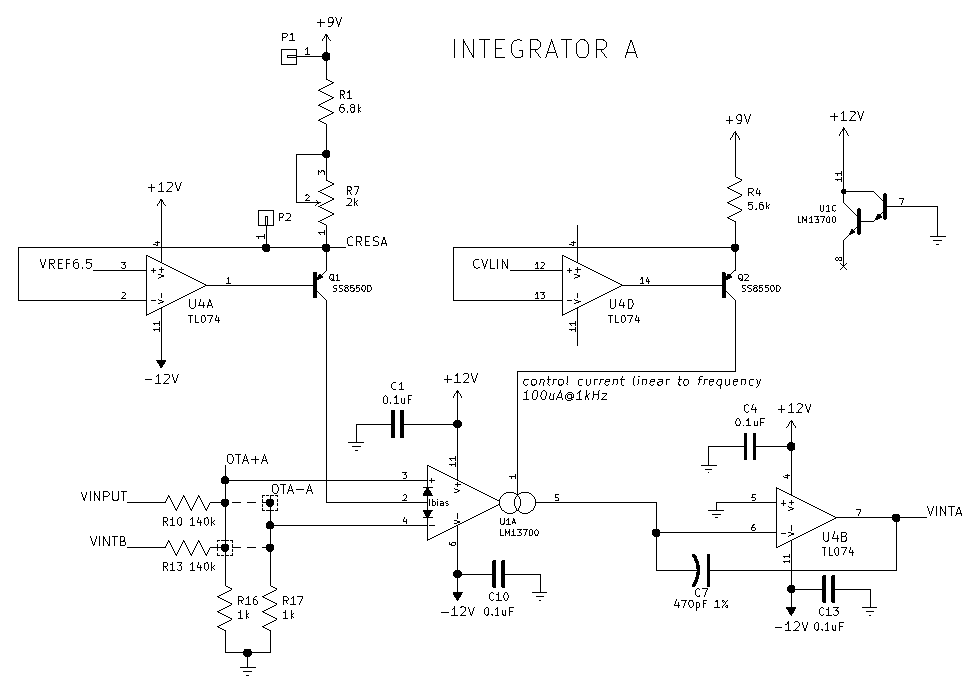
\includegraphics[width=\linewidth]{integrator}\par
\caption{One integrator in the filter core.}\label{fig:integrator}
\end{figure*}

This section's basic function is to integrate the difference between two
input voltages, multiplied by a global control voltage (applied to all the
integrators) and divided by a local time constant.  One half of an LM13700
(U1A) does the subtraction, multiplication, and division.  It needs its
input at a very low level for low distortion, so the input voltages
(nominally 10V peak to peak) go through 141:1 voltage dividers to bring them
down to about 71mV peak to peak.  Note the dotted lines on the schematic;
the PCB design offers a choice of pads so that R10 and R13 can each be
connected to either input of the operational transconductance amplifier. 
Normally, R13 would connect to the positive and R10 to the negative input,
providing an inversion (compare to the assignment of positive and negative
in the earlier explanations of the filter core) which will cancel out the
inversion of the integrator.

The LM13700 takes two control signals, both of which must be provided as
currents flowing into a pin held near some fixed voltage (either the
negative supply, or ground).  Both currents come from
op amp/PNP transistor sources, which generate currents proportional
to the difference between an input \emph{voltage} and the +9V supply. 
For the linearizing diode current, into pin 2, the ``control voltage'' is
actually a constant, the signal called VREF6.5.  It is really only
approximately 6.5V; its actual definition is one TL431 reference voltage
(should be close to 2.495V) less than the +9V supply (which is regulated by
a 78L09 and may be only approximately 9V).  The point is that the current
source, U4A and Q1, generate a stable constant current with a value
controlled by the sum of R1 and R7.  That is trimmed during adjustment to
set the constant coefficient for this integrator stage.  Other integrators
will have different resistances and therefore different diode currents, but
using this scheme to generate the diode currents ensures that the ratios
among the different integrator time constants will remain stable and can be
trimmed precisely.

The second control signal, into pin 1, comes from a similar op amp and PNP
transistor arrangement, but here it is controlled by the global signal
CVLIN, which is linear in the module's cutoff frequency, equal to the +9V
supply at 0Hz and decreasing (nominally) 0.560V/kHz.  The source that
generates this control voltage cannot go below ground, so the module's
global cutoff frequency is limited to about 16kHz.  The current source for
the integrator sources (to within the limits of its components) the current
that would flow through the 5.6k$\Omega$ resistor R4 if it were connected
between +9V and CVLIN, therefore 100$\mu$A per kHz.  However, the current
comes from the +9V supply and the op amp; it does not load up the CVLIN
line, which drives only the high-impedance input of the TL074 op amp.

With the two voltage and two current inputs, U1A generates a current output
on pin 5.  That is connected directly to the virtual ground on pin 6 of U4B,
the integrator.  Its output drives the other side of C7, the integrator
capacitor, to whatever voltage is needed to keep the virtual ground at
ground potential; thus except for the tiny bias current of the JFET-input op
amp, the current output from U1A directly charges and discharges C7,
providing a clean integrated voltage at the output of U4B.

The only remaining significant item in the integrator section is U1C, which
is one of the buffers built into the LM13700.  It is hooked up to do
nothing; using U4B for the integrator (and output buffer) renders the
LM13700's built-in buffer superfluous.

%%%%%%%%%%%%%%%%%%%%%%%%%%%%%%%%%%%%%%%%%%%%%%%%%%%%%%%%%%%%%%%%%%%%%%%%

\section{Output mixer}

Figure~\ref{fig:outmixer} shows the schematic for the output mixer, which
combines the integrator signals to generate the filter core output.  It is a
standard op amp sum/difference circuit, computing a linear combination of
the integrator outputs.  Each one has a trimmer for fine adjustment of its
coefficient in the sum.  Note that here, too, the dotted lines indicate
alternate pads on the PCB, allowing this board to be used to realize other
response curves by substituting component values and connections.  There are
also footprints provided (R28, R29, and R86) for components not needed in
the standard build, but which might possibly be used by other response
curves.

\begin{figure}
\centering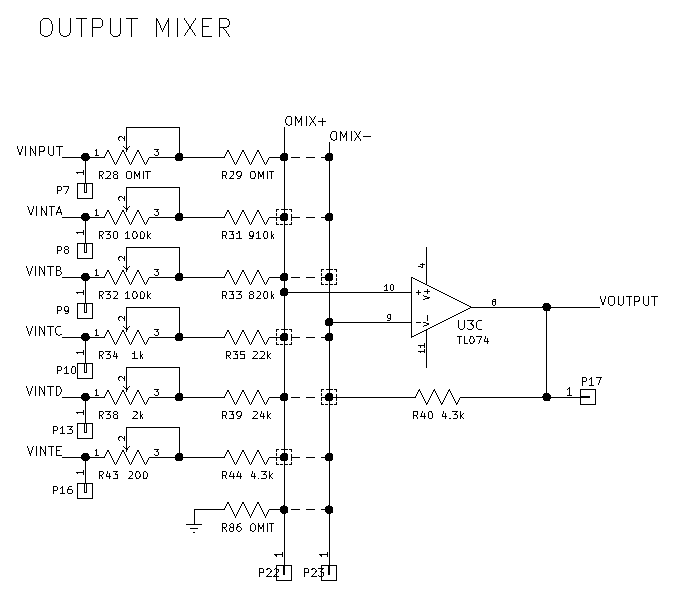
\includegraphics[width=\linewidth]{outmixer}\par
\caption{The output mixer.}\label{fig:outmixer}
\end{figure}

%%%%%%%%%%%%%%%%%%%%%%%%%%%%%%%%%%%%%%%%%%%%%%%%%%%%%%%%%%%%%%%%%%%%%%%%

\section{Control voltage processing}

Figure~\ref{fig:cvproc} shows the schematic for the control voltage
processing section.  This is a fairly conventional design.  There are
several exponentially-scaled inputs that all feed into the summing node of
the first op amp U10C:  V/octave input through J3 and R66; exponential FM
through J4, R64, and R69; coarse and fine tuning from the panel pots R81 and
R78 and the scaling resistors R74 and R74; and a constant offset controlled
by R88.

\begin{figure*}
\centering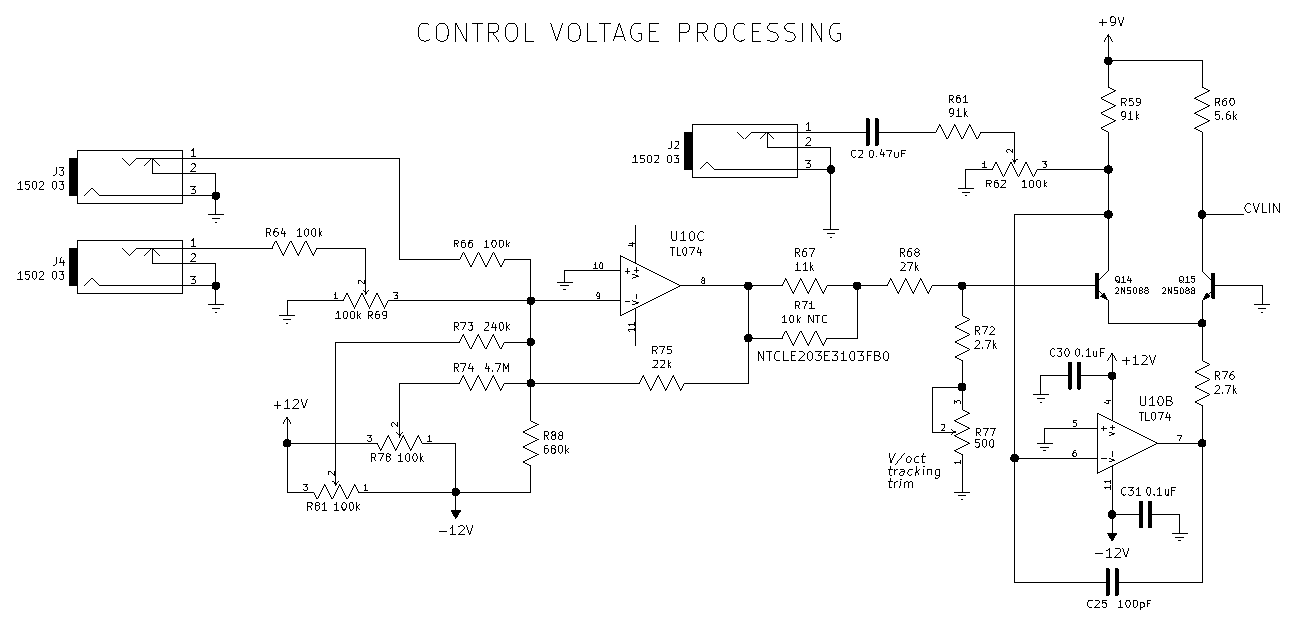
\includegraphics[width=\linewidth]{cvproc}\par
\caption{Control voltage processing.}\label{fig:cvproc}
\end{figure*}

Note that the exponential FM input is really just a second V/octave input with
an attenuation pot to allow it to be less sensitive than V/octave.  However,
because R64 and R66 might not match perfectly, the maximum-sensitivity
setting on this input may not be perfectly exactly 1V/octave.

With both of the tuning panel pots seeing a 24V range, using 240k$\Omega$ to
scale the coarse knob means it will have a range of ten octaves, and using
4.7M$\Omega$ on the fine tuning knob gives it a range of about half an
octave.

The 680k$\Omega$ offset resistor R88 was chosen by experiment with the
prototype.  It keeps the tuning knob range roughly where we want it; in
particular, it prevents the highest knob settings from hitting the hard
limit on control current.

All these exponential control signals go through U10C, which is a standard
inverting amplifier with a negative sub-unity gain.  Its output responds at
$-$220mV/octave.  Then R67, R68, R71, R72, and R77 are a
temperature-compensated voltage divider which reduces the control signal
further to about $-$18mV/octave, with the same temperature coefficient as a
silicon transistor (at least, as long as the ambient temperature is roughly
in the 15$^\circ$ to 30$^\circ$ range).  That scaled and
temperature-compensated exponential control signal is applied to
Q14.

What follows is a fairly standard two-transistor exponential current sink. 
The op amp U10B maintains a virtual ground on its negative input, pin 6.  To
do that, it must keep a constant current of 99$\mu$A flowing through Q14. 
The emitter of Q14 is therefore at its base voltage, minus whatever
base-to-emitter voltage it takes to make such a transistor pass 99$\mu$A.

Suppose the control voltage applied to the base of Q14 were zero.  Then Q14
and Q15 would see the same base-to-emitter voltage and each pass 99$\mu$A. 
CVLIN would then have a voltage 0.554V less than the +9V supply, the op amps
in the integrator control current sources would copy that voltage across
their own 5.6k$\Omega$ resistors, and the control currents would all be
99$\mu$A, making the module's nominal cutoff frequency 990Hz.

If the control voltages going into U10C are such as to drive the frequency
up an octave (1V added to the V/octave input, or equivalent changes to the
tuning knobs and FM input) then the base of Q14 will be driven down a
temperature-adjusted 18mV.  The op amp U10B pulls down its emitter
accordingly.  Then the base-to-emitter voltage of Q15, whose base is held
constant at 0V, is increasing by 18mV, which by the nature of NPN
transistors means its current must double.  Thus, the tuning goes up an
octave.  The same thing happens in reverse if the base of Q14 goes up 18mV;
then the current through Q15 is cut in half and the module tunes down an
octave.

The resistor R76 is chosen to keep the output voltage of U10B in a
comfortable range; higher resistance is better for stability, but we don't
want the op amp output to go too close to the rails in normal operation. 
Here, it will be at about $-$5.3V (1.6mA for Q15 and 0.1mA for Q14 going
through the 2.7k$\Omega$ resistor, plus about 0.7V for Q15's
base-to-emitter drop) when the control current hits its limit.

The capacitor value for C25 was chosen after taking some careful scope
measurements on a prototype of the circuit.  The thing is that op amps like
the TL074 are designed to guarantee stability when used at gains of at least
unity.  They are used with feedback loops typically composed of resistors,
which invariably have some insertion loss.  Insertion loss in the feedback
loop is equivalent to gain in the overall op amp circuit, and improves
stability.  Even an inverting op amp circuit like that around U10C which may
appear to have sub-unity gain has a greater than unity ``noise gain''
because of the loss in the feedback loop, and it is unconditionally stable. 
But in the case of U10B, we have Q14 in the feedback loop of the op amp
functioning as a common-base amplifier from the op amp's point of view, and
the gain of that amplifier will drive the op amp into instability unless we
do something about it.  Including C25 kills the loop gain at ultrasonic
frequencies (starting from about 100kHz) and prevents the op amp from going
into parasitic oscillation in the low megahertz range.

About the current limit:  note that CVLIN cannot go much below 0V because
the transistor will saturate and prevent its collector from going much below
its base.  That limits the current through R60, which is mirrored as the
control current to all the LM13700s, to about 1.6mA, safely below their
upper limit of 2.0mA.  Attempts to drive the module to higher frequencies
with higher control voltages will cause U10B to drive Q15 into
saturation and suck increasing amounts of current through its base, but the
power supply rails and R76 prevent that from being more than about 2 or 3mA,
which is safely within the transistor's capabilities.

Linear FM is applied through J2, AC-coupled through C2 and attenuated by
R62.  Whatever current we add or remove through this jack will be added to
or removed from the reference current passing through Q14; since the control
currents to the LM13700s all consist of this reference current multiplied by
the value set by the exponential control voltages, changing the reference
current has the effect of scaling the module's master frequency.  This is
not through-zero linear FM; the lowest possible frequency is zero.

%%%%%%%%%%%%%%%%%%%%%%%%%%%%%%%%%%%%%%%%%%%%%%%%%%%%%%%%%%%%%%%%%%%%%%%%

\section{VCA and feedback}

Figure~\ref{fig:vca} shows the schematic for the VCA and feedback subsystem. 
The VCA is a fairly standard LM13700 circuit using the one leftover
amplifier (three chips, six amplifiers, five needed for the filter
core).  As with the core VCAs, the LM13700's built-in buffer is connected to
do nothing.

\begin{figure*}
\centering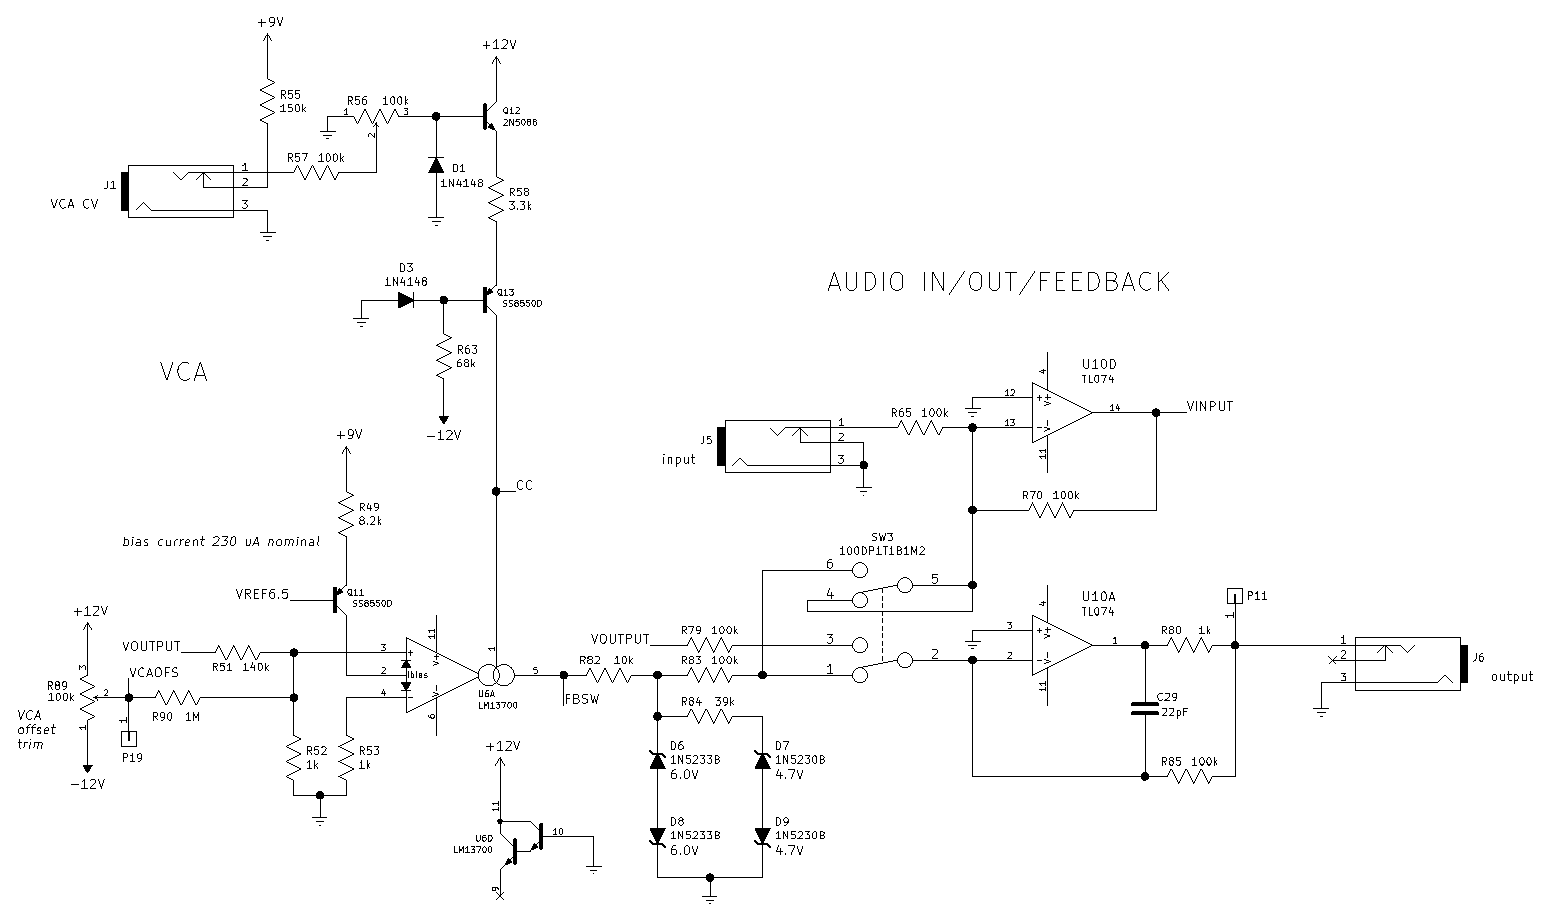
\includegraphics[width=\linewidth]{vca}\par
\caption{VCA and feedback.}\label{fig:vca}
\end{figure*}

Since accuracy is less critical at this point than in the core, we use just
a single transistor (Q11) as the source for the linearizing diode current instead of a
full op-amp-based precision current source.  The current is fixed at about
230$\mu$A.

The control voltage drives Q12, which is configured as an emitter follower,
to generate a current through R58 that will control the amplifier's gain
linearly.  The diode D1 is to protect the transistor against negative input
voltages, and the resistor network allows the attenuation knob to work and
makes the normalized input voltage when no cable is plugged in be equivalent
to about 5V (it is actually 9V, but with a high impedance that drops it down
to 5V).

D3 and R63 hold the base of Q13 at one diode drop below ground, so its
emitter is roughly at ground; since Q12's emitter is one diode drop below
its base, the overall voltage across R58 ends up being one diode drop less
than the unipolar control voltage.  At that level of approximation, it would
seem the VCA cuts out when the input voltage goes below about 0.6V.  In
fact, this effect is not sharp, because the ``diode drop'' from emitter to
base of these transistors is smaller when the current is very near zero; the
VCA will start to pass signal at a small fraction of a volt, but then enter
into its main linear behaviour at about 0.6V.  Part of the rationale for
this design is that we want to make sure it will fully ``close'' at zero
input; VCAs which pass some signal with zero control voltage get a lot of
complaints from users, and such behaviour would be especially annoying in
the case of this filter, with its attempt at a brick-wall frequency
response.

The VCA output goes through a Zener-diode clipping circuit that provides two
levels of clipping, soft at about $\pm$5.3V (4.7V Zener voltage from 0.6V
for the other, forward-biased, diode) and hard at about $\pm$6.6V.  This is
meant to provide both a clean gain roll-off when the module is
used as an oscillator, and some ``warmth'' and reasonable limits on output
level in filter mode when the built-in VCA is used.  The sharp response
cutoff makes output level especially unpredictable for this filter compared
to other common synth filters.

The mode switch SW3 selects how the VCA will be connected.  It can be in the
output path, in which case the input buffer takes its input only from the
module input jack J5, and the output buffer takes its input from the VCA. 
The other setting uses the VCA for feedback.  Then the VCA output goes to
the input buffer, and the output buffer is driven directly by the filter
core's output mixer.

The input buffer is a very much standard negative-unity-gain inverting
amplifier.  It provides a well-behaved impedance to the outside world, sums
the input signal with any feedback from the VCA when in feedback mode, and
provides the 180$^\circ$ phase shift needed to support oscillation.  The
output buffer is a similar circuit adapted for driving a cable and
another module's input: it has an in-the-loop current limiting resistor to
protect against short circuit, and a 22pF capacitor for phase compensation.

%%%%%%%%%%%%%%%%%%%%%%%%%%%%%%%%%%%%%%%%%%%%%%%%%%%%%%%%%%%%%%%%%%%%%%%%

\section{Power inlet and reference generator}

Figure~\ref{fig:powerref} shows the schematic for the power- and
voltage-handling circuitry.

\begin{figure}
\centering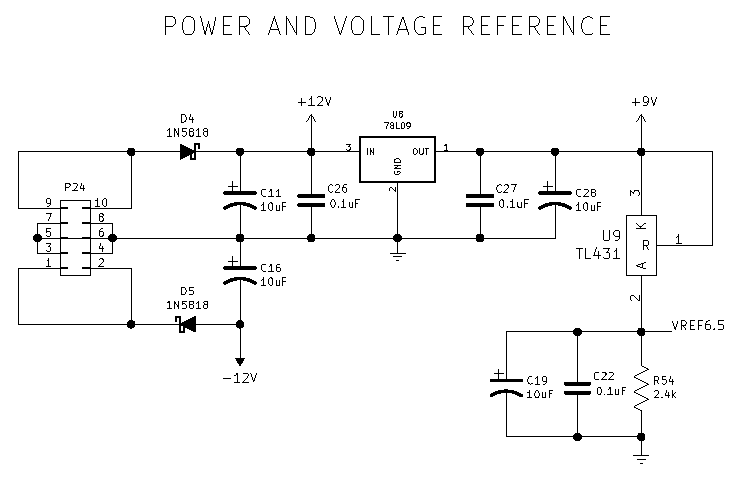
\includegraphics[width=\linewidth]{powerref}\par
\caption{Power handling and reference voltage section}\label{fig:powerref}
\end{figure}

Power from the Eurorack power connector P24 goes through two Schottky diodes
for reverse-connection protection, and is filtered by a pair of 10$\mu$F
capacitors before going to power all parts of the module.  Control currents
are all sourced out of a local $+$9V supply regulated by a 78L09 chip, both
to keep them as clean as possible and so that op amp outputs can comfortably
approach this supply voltage.  There is also a reference voltage called
VREF6.5, which is defined to be one TL431 drop (of 2.495V) less than the
$+$9V supply.  The constant difference between VREF6.5 and $+$9V is used as
a reference by the constant-current sources for LM13700 linearizing-diode
currents; they drive resistors to voltage drops matching this difference.
